\documentclass[11pt,reqno]{amsart}

\usepackage[T1]{fontenc}
\usepackage{lmodern}
\usepackage{amsmath,amssymb,amsthm,mathtools}
\usepackage{booktabs}
\usepackage{graphicx}
\usepackage{enumitem}
\usepackage[margin=1.15in]{geometry}
\usepackage{microtype}
\usepackage[dvipsnames]{xcolor}
\usepackage[colorlinks=true,linkcolor=MidnightBlue,citecolor=MidnightBlue,urlcolor=MidnightBlue]{hyperref}

\newtheorem{theorem}{Theorem}[section]
\newtheorem{proposition}[theorem]{Proposition}
\newtheorem{lemma}[theorem]{Lemma}
\newtheorem{corollary}[theorem]{Corollary}
\theoremstyle{definition}
\newtheorem{definition}[theorem]{Definition}
\theoremstyle{remark}
\newtheorem{remark}[theorem]{Remark}

\numberwithin{equation}{section}

\newcommand{\R}{\mathbb{R}}
\newcommand{\C}{\mathbb{C}}
\newcommand{\N}{\mathbb{N}}
\newcommand{\Z}{\mathbb{Z}}
\newcommand{\dd}{\mathrm{d}}
\newcommand{\ii}{\mathrm{i}}
\newcommand{\ee}{\mathrm{e}}
\newcommand{\Rea}{\mathrm{Re}}
\newcommand{\Ima}{\mathrm{Im}}
\newcommand{\sinchyp}{\mathrm{sinc}_{\mathrm{hyp}}}

\title[Logarithmic Dilation and Saddle-Point Shell Structure]{Logarithmic Dilation of the Jacobi--Riemann Kernel, Strip-Holomorphic Shell Partitions, Stieltjes Diagonal Asymptotics, and Off-Diagonal Obstructions}

\author{Thijs Missiaen}
\address{Independent Researcher, Belgium (ORCID: \href{https://orcid.org/0009-0007-3678-0810}{0009-0007-3678-0810})}
\email{thijs.missiaen@gmail.com}
\date{November 2026}
\subjclass[2020]{Primary 11M06, 41A60; Secondary 30D15, 33B15}
\keywords{Riemann $\Xi$-function, transverse Wronskian, Jacobi theta kernel, logarithmic shell dilation, Spira modulus inequality, Riemann--Siegel remainder, Stieltjes constants}

\begin{document}

\begin{abstract}
We analyze the logarithmic shell structure of Riemann's Jacobi theta kernel $\Phi(u) = \sum_{m=1}^{\infty} \phi_m(u)$ governing the canonical transverse Wronskian $W(d,t) = \frac{1}{2}\partial_d\lvert\Xi(t - \ii d)\rvert^2 = 16\int_0^{\infty} y\sinh(2dy)I(y,t)\,\dd y$. Every shell $\phi_m(u) = m^{-1/2}\varphi_1(u + \frac{1}{2}\ln m)$ is an exact logarithmic translation of $\varphi_1(w)$ whose bilateral Laplace--Mellin transform $\mathcal{G}(s) = \frac{1}{8}s(s-1)\pi^{-s/2}\Gamma(s/2)$ satisfies $(1-s)(-s) \equiv s(s-1)$ on $\C$; combined with the Spira and Saidak--Zvengrowski functional-equation modulus inequality $\lvert\chi(s)\rvert < 1$, this yields strict branch damping across active Riemann--Siegel modes $1 \le n \le N(t) = \lfloor\sqrt{t/2\pi}\rfloor$. We show that previously proposed $\sinh(8z)$ cutoff weights introduce poles at $\lvert\Ima(z)\rvert = \frac{\pi}{48} < \frac{\pi}{8}$, whereas both the weight-free even remainder kernel $R_N^{\mathrm{ker}}(z)$ and the logistic partition $w_4(z) = (1+\ee^{-8z})^{-1}$ remain pole-free throughout $\lvert\Ima(z)\rvert < \frac{\pi}{8}$. Finally, we prove a cubic-logarithmic Stieltjes diagonal expansion and a sharp $\mathcal{O}(t^{-3/2})$ bound for the boundary pair $(N-1,N)$, while showing that the $\binom{N(t)}{2}$ off-diagonal pairs sum in $L^1$ to $\asymp t^{1/2}$ and overwhelm the diagonal pointwise.
\end{abstract}

\maketitle

\section{Introduction and Main Results}\label{sec:intro}

In Riemann's memoir~\cite{riemann1859}, the completed zeta function $\xi(s) := \frac{1}{2}s(s-1)\pi^{-s/2}\Gamma(s/2)\zeta(s)$ is rotated to the spectral variable $z = t - \ii d$ ($s = \frac{1}{2} + \ii z = \frac{1}{2} + d + \ii t$) via the even entire function $\Xi(z) := \xi(\frac{1}{2} + \ii z)$. Using Jacobi's transformation law~\cite{jacobi1829} for $\theta(x) = \sum_{m=-\infty}^{\infty} \ee^{-\pi m^2 x}$, $\Xi(z)$ admits the Fourier cosine representation~\cite{polya1926,titchmarsh1986}
\begin{equation}\label{eq:Xi_jacobi_intro}
\Xi(z) = 8\int_0^{\infty} \Phi(u)\cos(2zu)\,\dd u = 4\int_{-\infty}^{\infty} \Phi(u)\cos(2zu)\,\dd u, \qquad \Phi(u) := \sum_{m=1}^{\infty} \phi_m(u),
\end{equation}
where each shell $\phi_m(u) := (2\pi^2 m^4 \ee^{9u} - 3\pi m^2 \ee^{5u})\exp(-\pi m^2 \ee^{4u})$ is holomorphic on $\C$, while $\Phi(u) = \Phi(-u)$ is even on $\R$ and holomorphic in the open strip $\lvert\Ima(u)\rvert < \frac{\pi}{8}$. Writing $\Xi(t - \ii d) = R(d,t) + \ii I(d,t)$ for real $(d,t)$, the Cauchy--Riemann equations $R_d = I_t$ and $I_d = -R_t$ identify the canonical transverse Wronskian~\cite{speiser1934,lagarias1999,hinkkanen1997,csordas1986} with the Wigner phase-space integral~\cite{wigner1932,hudson1974}
\begin{equation}\label{eq:W_canonical_intro}
\boxed{W(d,t) := \frac{1}{2}\frac{\partial}{\partial d}\bigl\lvert\Xi(t - \ii d)\bigr\rvert^2 = R(d,t)I_t(d,t) - I(d,t)R_t(d,t) = 16\int_0^{\infty} y\sinh(2dy)\,I(y,t)\,\dd y,}
\end{equation}
where $I(y,t) := \int_{-\infty}^{\infty} \Phi(\frac{x+y}{2})\Phi(\frac{x-y}{2})\cos(2tx)\,\dd x$ is even in $y$ and $\widetilde{W}(d,t) := W(d,t)/d$.

Connecting the continuum representation~\eqref{eq:W_canonical_intro} to the finite Riemann--Siegel Dirichlet sum of length $N(t) := \lfloor\sqrt{t/2\pi}\rfloor$~\cite{siegel1932,gabcke1979} requires care at four distinct analytical points:
\begin{enumerate}[label=\textup{(\arabic*)},leftmargin=2.2em]
\item \textit{Archimedean reflection versus collective Dirichlet zeros.} Individual shells generate symmetric pairs $\mathcal{G}(s)m^{-s} + \mathcal{G}(1-s)m^{-(1-s)}$. Clarifying how $\lvert\mathcal{G}(1-s)/\mathcal{G}(s)\rvert = \lvert\chi(s)\rvert < 1$ follows from classical results of Spira~\cite{spira1965} and Saidak--Zvengrowski~\cite{saidakzvengrowski2003} separates single-shell Archimedean convexity from collective zero cancellation.
\item \textit{Strip holomorphy of symmetrized shells.} Naive half-line symmetrization $\phi_m(\lvert u\rvert)$ creates an odd-derivative jump at $u = 0$, whereas aggressive double-exponential cutoffs such as $(1 + \exp(-2\pi\sinh(8z)))^{-1}$ introduce poles inside $\lvert\Ima(z)\rvert < \frac{\pi}{8}$ at $\lvert\Ima(z)\rvert = \frac{\pi}{48}$.
\item \textit{Diagonal asymptotics versus off-diagonal multiplicity.} On the diagonal $m = n$, phase cancellation produces a positive $(\ln t)^3$ Stieltjes expansion and the single boundary pair $(N-1,N)$ is $\mathcal{O}(t^{-3/2})$, yet the $\binom{N(t)}{2} \asymp t$ off-diagonal cross-pairs sum in $L^1$ to $\asymp t^{1/2}$ and dominate pointwise whenever phases align.
\item \textit{Contour tail bounds and remainder domains.} Unsplit $\cosh(2(d+\ii t)(\xi+\ii\eta))$ tail integrals introduce an artificial $\cosh(2t\eta)$ factor, whereas Gabcke's explicit remainder theorem~\cite{gabcke1979} applies strictly on $d = 0$ for $t \ge 200$ after subtracting the leading saddle term $\Psi(p)$.
\end{enumerate}

The purpose of this paper is to establish the exact identities governing items~(1)--(4) while delineating the analytical obstructions cleanly and without overclaiming.

\begin{theorem}[Summary of Exact Shell Identities and Analytical Boundaries]\label{thm:main_summary}
Let $d \in (0, \frac{1}{2}]$, $t \ge 7$, $z = t - \ii d$, $s = \frac{1}{2} + d + \ii t$, and $N(t) = \lfloor\sqrt{t/2\pi}\rfloor$.
\begin{enumerate}[label=\textup{(\roman*)},leftmargin=2.2em]
\item \textbf{Logarithmic Dilation and Spira Branch Damping.} Every shell satisfies $\phi_m(u) = m^{-1/2}\varphi_1(u + \frac{1}{2}\ln m)$ with $\varphi_1(w) := (2\pi^2\ee^{9w} - 3\pi\ee^{5w})\ee^{-\pi\ee^{4w}}$ and bilateral Laplace--Mellin transform $\mathcal{G}(s) = \frac{1}{8}s(s-1)\pi^{-s/2}\Gamma(s/2)$ ($\Rea(s) > -2$). Since $(1-s)(-s) \equiv s(s-1)$ on $\C$, $\rho_\Gamma(d,t) := \lvert\mathcal{G}(1-s)/\mathcal{G}(s)\rvert = \lvert\chi(s)\rvert < \ee^{-2d\vartheta'(t)} < 1$ for all $d \in (0, \frac{1}{2}]$ and $t \ge 7$~\cite{spira1965,saidakzvengrowski2003}, whence $\rho_\Gamma(d,t)n^{2d} < \ee^{-2d\omega_n(t)} < 1$ for $n = 1$ ($t \ge 7$), for every $1 \le n \le N(t) - 1$ ($t \ge 8\pi$), and for $n = N(t)$ whenever $\ln N(t) < \vartheta'(t)$.
\item \textbf{Strip-Holomorphic Symmetrization and Exact Remainder Kernel.} The weight $w_{\mathrm{Jac}}(z) = (1 + \exp(-2\pi\sinh(8z)))^{-1}$ has poles at $z = \pm\ii\frac{\pi}{48}$ inside $\lvert\Ima(z)\rvert < \frac{\pi}{8}$. By contrast, the weight-free even remainder kernel $R_N^{\mathrm{ker}}(z) := \Phi(z) - \sum_{m=1}^N [\phi_m(z) + \phi_m(-z)]$ and the logistic shells $\Phi_m^{\mathrm{log}}(z) := w_4(z)\phi_m(z) + w_4(-z)\phi_m(-z)$ with $w_4(z) := (1 + \ee^{-8z})^{-1}$ are holomorphic throughout the full open strip $\lvert\Ima(z)\rvert < \frac{\pi}{8}$ and satisfy $(R_N^{\mathrm{ker}})^{(2k+1)}(0) = (\Phi_m^{\mathrm{log}})^{(2k+1)}(0) = 0$ for all $k \ge 0$.
\item \textbf{Stieltjes Diagonal Expansion, $(N-1,N)$ Self-Damping, and Off-Diagonal Scaling.} With $L := 2\vartheta'(t) = \ln(t/2\pi) + \mathcal{O}(t^{-2})$, the critical-line main-sum diagonal satisfies $\mathcal{D}_{\mathrm{diag}}(0,t) := \sum_{n=1}^{N(t)} \frac{4\omega_n(t)^2}{n} = \frac{1}{6}L^3 + \gamma_{\mathrm{E}}L^2 - 4\gamma_1^{\mathrm{St}}L + 4\gamma_2^{\mathrm{St}} + \mathcal{O}(t^{-3/2}\ln^2 t)$, and for $t \ge 8\pi$ ($N = N(t) \ge 2$) the adjacent boundary pair obeys $0 < A_{N-1,N}(0,t) < \frac{(3N-2)^2}{[N(N-1)]^{5/2}} < \frac{9}{(N-1)^3} = \mathcal{O}(t^{-3/2})$. However, the total $L^1$ amplitude of all $\binom{N(t)}{2} \sim \frac{t}{4\pi}$ off-diagonal pairs scales as $\sum_{1 \le m < n \le N(t)} 2A_{m,n}(0,t) = \frac{96}{\sqrt{2\pi}}\,t^{1/2} + \mathcal{O}((\ln t)^2 t^{1/4}) \gg \mathcal{D}_{\mathrm{diag}}(0,t)$.
\item \textbf{Unshifted Real-Axis Tail Bound and Hyperbolic Sinc Ratio.} On the real half-line $\eta = 0$, the evanescent tail integral $\mathcal{I}_{\mathrm{tail}}(N,z,0) := \sum_{m=N+1}^{\infty} \int_0^{\infty} \phi_m(\xi)\allowbreak\cos(2z\xi)\,\dd\xi$ satisfies $\lvert\mathcal{I}_{\mathrm{tail}}(N,z,0)\rvert \le b_{N+1}(d,0)/(1 - q_N(0))$ without artificial $\cosh(2t\eta)$ growth, while $\sinchyp(dL/2)/\sinchyp(dL) \equiv \cosh(dL/2)^{-1} \le 2(t/2\pi)^{-d/2}$.
\end{enumerate}
\end{theorem}

\subsection{Proof overview}\label{subsec:proof_overview}

The proofs rest on three analytical ingredients:
\begin{enumerate}[label=\textup{(\arabic*)},leftmargin=2.2em]
\item \textit{Logarithmic shift-equivariance and tetragamma convexity (Section~\ref{sec:dilation}).} Substituting $v = u + \frac{1}{2}\ln m$ reduces the bilateral Mellin integral of $\phi_m$ to $\mathcal{G}(s)m^{-s}$. Because $(1-s)(-s) = s(s-1)$ identically, $\lvert\mathcal{G}(1-s)/\mathcal{G}(s)\rvert$ reduces to $\lvert\chi(s)\rvert$, whose radial decay on $d \in (0, \frac{1}{2}]$ follows from positivity of the digamma carrier $\mathcal{A}_\Gamma(0,t) = \vartheta'(t)$ above $t_{\mathrm{crit}} \approx 6.289836$ and positive real part of the tetragamma derivative $\psi''$~\cite{olver1997,spira1965,saidakzvengrowski2003}.
\item \textit{Pole localization in $\lvert\Ima(z)\rvert < \frac{\pi}{8}$ (Section~\ref{sec:shells}).} Solving $1 + \ee^{-8z} = 0$ places all poles of $w_4(z)$ at $\Ima(z) = \frac{2k+1}{8}\pi$ outside $\lvert\Ima(z)\rvert < \frac{\pi}{8}$, whereas $2\pi\sinh(8z) = \pm\ii\pi$ places poles of $w_{\mathrm{Jac}}(z)$ at $\Ima(z) = \pm\frac{\pi}{48}$. Simultaneously, rewriting the finite bilateral main sum over $[0, \infty)$ isolates the weight-free even remainder kernel $R_N^{\mathrm{ker}}(z)$.
\item \textit{Euler--Maclaurin boundary vanishing and real-axis incomplete-Gamma integration by parts (Sections~\ref{sec:stieltjes}--\ref{sec:tails}).} Because $f(x) = (\frac{1}{2}L - \ln x)^2/x$ satisfies $f(\ee^{L/2}) = f'(\ee^{L/2}) = 0$, fractional-part jumps at $N(t) = \lfloor\ee^{L/2}\rfloor$ vanish to second order in $\mathcal{D}_{\mathrm{diag}}(0,t)$, while substituting $w = \ee^{4\xi} \ge 1$ bounds the $u \ge 0$ tail geometrically.
\end{enumerate}

\subsection{Notation and canonical normalizations}\label{subsec:notation}

Throughout, $s = \sigma + \ii t$ with $\sigma = \frac{1}{2} + d$, $z = t - \ii d$, $\xi(s) = \frac{1}{2}s(s-1)\pi^{-s/2}\Gamma(s/2)\zeta(s) = 4\mathcal{G}(s)\zeta(s)$, and $\Xi(z) = \xi(\frac{1}{2} + \ii z)$. Note that writing $\widetilde{\Phi}(\tilde{u}) := 2\Phi(\tilde{u}/2)$ translates~\eqref{eq:Xi_jacobi_intro} into $\Xi(z) = 2\int_0^{\infty} \widetilde{\Phi}(\tilde{u})\cos(z\tilde{u})\,\dd\tilde{u}$; we work uniformly in the $(u, 2zu)$ variable of~\eqref{eq:Xi_jacobi_intro}--\eqref{eq:W_canonical_intro}. We set $\vartheta(t) := \Ima\ln\Gamma(\frac{1}{4} + \ii\frac{t}{2}) - \frac{t}{2}\ln\pi$, $\omega_n(t) := \vartheta'(t) - \ln n$, $L := 2\vartheta'(t)$, $N(t) := \lfloor\sqrt{t/2\pi}\rfloor$, and $\sinchyp(x) := \frac{\sinh x}{x}$ ($\sinchyp(0) := 1$). The Stieltjes constants~\cite{stieltjes1885} are defined by $\zeta(1+s) = s^{-1} + \sum_{k=0}^{\infty} \frac{(-1)^k}{\Gamma(k+1)}\gamma_k^{\mathrm{St}} s^k$ with $\gamma_0^{\mathrm{St}} = \gamma_{\mathrm{E}}$.

\section{Logarithmic Dilation and the Spira--Saidak--Zvengrowski Modulus Inequality}\label{sec:dilation}

\begin{proposition}[Logarithmic Dilation and Bilateral Laplace--Mellin Transform]\label{prop:dilation}
Define the generating shell on $\C$ by $\varphi_1(w) := (2\pi^2\ee^{9w} - 3\pi\ee^{5w})\exp(-\pi\ee^{4w})$. Then:
\begin{enumerate}[label=\textup{(\roman*)},leftmargin=2.2em]
\item For every integer $m \ge 1$ and all $u \in \C$, $\phi_m(u) = m^{-1/2}\varphi_1(u + \frac{1}{2}\ln m)$. On $\R$, $\varphi_1(w)$ has a unique zero at $w_{\mathrm{node}} = \frac{1}{4}\ln(\frac{3}{2\pi}) \approx -0.1848161944$, a global maximum at $w_{\max} = \frac{1}{4}\ln(\frac{15+\sqrt{105}}{8\pi}) \approx +0.0011334898$, and a global minimum at $w_{\min} = \frac{1}{4}\ln(\frac{15-\sqrt{105}}{8\pi}) \approx -0.4163462679$.
\item For $\Rea(s) > -2$, the bilateral Laplace--Mellin integral converges absolutely to
\begin{equation}\label{eq:G_mellin_exact}
\mathcal{G}(s) := \int_{-\infty}^{\infty} \varphi_1(v)\,\ee^{2(s - 1/2)v}\,\dd v = \frac{1}{8}s(s-1)\pi^{-s/2}\Gamma\!\left(\frac{s}{2}\right),
\end{equation}
and extends meromorphically to $\C$ with $\xi(s) = 4\mathcal{G}(s)\zeta(s)$. Consequently, for every $m \ge 1$ and $z = t - \ii d$ ($s = \frac{1}{2} + d + \ii t$),
\begin{equation}\label{eq:Fm_bilateral}
F_{m,\pm}(z) := 2\int_{-\infty}^{\infty} \phi_m(u)\cos(2zu)\,\dd u = \mathcal{G}(s)m^{-s} + \mathcal{G}(1-s)m^{-(1-s)}.
\end{equation}
\end{enumerate}
\end{proposition}

\begin{proof}
(i) Since $\ee^{k(u + \frac{1}{2}\ln m)} = m^{k/2}\ee^{ku}$, we have $m^{-1/2}\varphi_1(u + \frac{1}{2}\ln m) = m^{-1/2}(2\pi^2 m^{9/2}\ee^{9u} - 3\pi m^{5/2}\ee^{5u})\exp(-\pi m^2\ee^{4u}) = \phi_m(u)$. Setting $X := \pi\ee^{4w} > 0$, $\varphi_1(w) = 0 \iff 2X = 3$, while $\varphi_1'(w) = 0 \iff 8X^2 - 30X + 15 = 0 \iff X = \frac{15 \pm \sqrt{105}}{8}$.

(ii) As $v \to -\infty$, $\varphi_1(v)\ee^{(2s-1)v} \sim -3\pi\ee^{(2s+4)v}$, which is integrable for $\Rea(s) > -2$, while $\exp(-\pi\ee^{4v})$ gives super-exponential decay as $v \to +\infty$. Substituting $x = \pi\ee^{4v}$ ($\dd v = \frac{\dd x}{4x}$) gives
\[
\mathcal{G}(s) = \frac{\pi^{-s/2}}{4}\int_0^{\infty} \bigl(2x^{s/2+1} - 3x^{s/2}\bigr)\ee^{-x}\,\dd x = \frac{\pi^{-s/2}}{4}\left[2\Gamma\!\left(\frac{s}{2}+2\right) - 3\Gamma\!\left(\frac{s}{2}+1\right)\right],
\]
which simplifies via $\Gamma(w+1) = w\Gamma(w)$ to $\frac{1}{4}\pi^{-s/2}\frac{s}{2}(\frac{s}{2} - \frac{1}{2})\Gamma(\frac{s}{2}) = \frac{1}{8}s(s-1)\pi^{-s/2}\Gamma(\frac{s}{2})$. Writing $2\cos(2zu) = \ee^{2(s-1/2)u} + \ee^{2((1-s)-1/2)u}$ and substituting $v = u + \frac{1}{2}\ln m$ yields~\eqref{eq:Fm_bilateral}.
\end{proof}

We now connect~\eqref{eq:Fm_bilateral} to the classical functional-equation factor $\chi(s) := \pi^{s-1/2}\Gamma(\frac{1-s}{2})/\Gamma(\frac{s}{2})$ studied by Spira~\cite{spira1965} and Saidak and Zvengrowski~\cite{saidakzvengrowski2003}.

\begin{proposition}[Spira--Saidak--Zvengrowski Branch Damping]\label{prop:spira_damping}
Let $s = \frac{1}{2} + d + \ii t$ ($d > 0$, $t \ge 7$). Set $\mathcal{A}_\Gamma(d,t) := \frac{1}{2}\Rea\,\psi(\frac{1}{4} + \allowbreak\frac{d}{2} + \allowbreak\ii\frac{t}{2}) - \frac{1}{2}\ln\pi$ and $\mathcal{A}_\Gamma^{\mathrm{sym}}(d,t) := \frac{1}{2}[\mathcal{A}_\Gamma(d,t) + \allowbreak\mathcal{A}_\Gamma(-d,t)]$. Then:
\begin{enumerate}[label=\textup{(\roman*)},leftmargin=2.2em]
\item By elementary algebra, $(1-s)(-s) = s^2 - s \equiv s(s-1)$ holds identically for all $s \in \C$. Hence the polynomial prefactor cancels identically in $\mathcal{G}(1-s)/\mathcal{G}(s) = \chi(s)$, and
\begin{equation}\label{eq:rho_gamma_exact}
\rho_\Gamma(d,t) := \left\lvert\frac{\mathcal{G}(1-s)}{\mathcal{G}(s)}\right\rvert = \lvert\chi(s)\rvert = \pi^d\left\lvert\frac{\Gamma(\frac{1}{4} - \frac{d}{2} + \ii\frac{t}{2})}{\Gamma(\frac{1}{4} + \frac{d}{2} + \ii\frac{t}{2})}\right\rvert = \exp\!\left(-2\int_0^d \mathcal{A}_\Gamma^{\mathrm{sym}}(u,t)\,\dd u\right).
\end{equation}
\item For all $t > t_{\mathrm{crit}} = 6.28983598883690277967\dots$ (in particular $t \ge 7$) and $d \in (0, \frac{1}{2}]$, $\mathcal{A}_\Gamma^{\mathrm{sym}}(u,t) > \mathcal{A}_\Gamma(0,t) = \vartheta'(t) > 0$ for $u \in (0, d]$, so $\rho_\Gamma(d,t) < \ee^{-2d\vartheta'(t)} < 1$~\cite{spira1965,saidakzvengrowski2003}.
\item For $d \in (0, \frac{1}{2}]$, every mode $n = 1$ ($t \ge 7$) and $1 \le n \le N(t) - 1$ ($t \ge 8\pi$) satisfies $\omega_n(t) = \vartheta'(t) - \ln n > 0$ and the strict branch-damping inequality
\begin{equation}\label{eq:branch_damping}
\rho_\Gamma(d,t)\,n^{-1/2+d} < \ee^{-2d\omega_n(t)}\,n^{-1/2-d} < n^{-1/2-d},
\end{equation}
which also holds at $n = N(t)$ whenever $\ln N(t) < \vartheta'(t)$ (outside the transition micro-intervals $2\pi m^2 \le t < t_m^*$ where $\vartheta'(t_m^*) = \ln m$ and $\omega_m(t) \in (-\frac{1}{24t^2}, 0]$).
\end{enumerate}
\end{proposition}

\begin{proof}
(i) Dividing $\mathcal{G}(1-s) = \frac{1}{8}(1-s)(-s)\pi^{-(1-s)/2}\Gamma(\frac{1-s}{2})$ by $\mathcal{G}(s)$ and using $(1-s)(-s) = s(s-1)$ gives $\mathcal{G}(1-s)/\mathcal{G}(s) = \chi(s)$. Since $\partial_u\ln\lvert\Gamma(\frac{1}{4} \pm \frac{u}{2} + \ii\frac{t}{2})\rvert = \pm\frac{1}{2}\Rea\,\psi(\frac{1}{4} \pm \frac{u}{2} + \ii\frac{t}{2})$ and $\ln\lvert\Gamma(\bar{w})\rvert = \ln\lvert\Gamma(w)\rvert$, integrating $\partial_u\ln\rho_\Gamma(u,t) = -2\mathcal{A}_\Gamma^{\mathrm{sym}}(u,t)$ from $0$ to $d$ with $\rho_\Gamma(0,t) = 1$ yields~\eqref{eq:rho_gamma_exact}.

{\sloppy
(ii) By Stirling's series with Olver's remainder~\cite{olver1997}, $\vartheta'(t) = \frac{1}{2}\ln(\frac{t}{2\pi}) + \mathcal{O}(t^{-2})$ crosses zero uniquely at $t_{\mathrm{crit}} \approx 6.289836 < 7$. Moreover, $\partial_u^2\mathcal{A}_\Gamma^{\mathrm{sym}}(u,t) = \frac{1}{16}[\Rea\,\psi''(\frac{1}{4}+\frac{u}{2}+\ii\frac{t}{2}) + \Rea\,\psi''(\frac{1}{4}-\frac{u}{2}+\ii\frac{t}{2})]$. For $w = x + \ii y$ with $x \in [0, \frac{1}{2}]$ and $y = \frac{t}{2} \ge \frac{7}{2}$, set $w_1 := w + 1 = x_1 + \ii y$ ($x_1 \in [1, \frac{3}{2}]$), so $\psi''(w) = \psi''(w_1) - 2w^{-3}$. Since $0 \le x < x_1 \le \frac{3}{2} < \sqrt{3}\,y$, both $\Rea(-2w^{-3}) = 2x(3y^2-x^2)\lvert w\rvert^{-6} \ge 0$ and $\Rea(-w_1^{-3}) > 0$. Applying second-order Euler--Maclaurin summation to $\psi''(w_1) = -2\sum_{k=0}^{\infty}(w_1+k)^{-3}$ gives $\psi''(w_1) = -w_1^{-2} - w_1^{-3} + R_2(w_1)$, where $R_2(w_1) = -12\int_0^{\infty}\{\tau\}(1-\{\tau\})(w_1+\tau)^{-5}\,\dd\tau$ obeys $\lvert R_2(w_1)\rvert \le 3\int_0^{\infty}((x_1+\tau)^2+y^2)^{-5/2}\,\dd\tau < 3y^{-4}\int_0^{\infty}(s^2+1)^{-5/2}\,\dd s = 2y^{-4}$. Since $\Rea(-w_1^{-2}) = (y^2-x_1^2)(x_1^2+y^2)^{-2} \ge (y^2 - \frac{9}{4})(y^2 + \frac{9}{4})^{-2} > 2y^{-4}$ for all $y \ge \frac{7}{2}$ (as $y^2(y^4 - \frac{17}{4}y^2 - 9) - \frac{81}{8} \ge \frac{8641}{8} > 0$), we obtain $\Rea\,\psi''(w) > 0$, hence $\partial_u^2\mathcal{A}_\Gamma^{\mathrm{sym}}(u,t) > 0$. Because $\partial_u\mathcal{A}_\Gamma^{\mathrm{sym}}(0,t) = 0$, $\mathcal{A}_\Gamma^{\mathrm{sym}}(u,t) > \vartheta'(t) > 0$ on $(0, d]$, proving $\rho_\Gamma(d,t) < \ee^{-2d\vartheta'(t)} < 1$.\par}

{\sloppy
(iii) For $t \ge 7$, $\omega_1(t) = \vartheta'(t) > 0$. For $t \ge 8\pi$ ($N = N(t) \ge 2$), Olver's remainder bound~\cite[Ch.~8]{olver1997} gives $\vartheta'(t) > \frac{1}{2}\ln(\frac{t}{2\pi}) - \frac{1}{24t^2} \ge \ln N - \frac{1}{24t^2}$. Thus for $1 \le n \le N - 1$, $\omega_n(t) \ge \omega_{N-1}(t) > \ln(\frac{N}{N-1}) - \frac{1}{24t^2} > \frac{1}{N} - \frac{1}{96\pi^2 N^4} > 0$, and at $n = N$ the inequality $\omega_N(t) > 0$ holds whenever $\ln N < \vartheta'(t)$, giving~\eqref{eq:branch_damping}.\par}
\end{proof}

\begin{remark}[Single-shell positivity versus Davenport--Heilbronn counterexamples]\label{rem:davenport_heilbronn}
For $m = 1$, $F_{1,\pm}(z) = \mathcal{G}(s) + \mathcal{G}(1-s)$ satisfies $\lvert F_{1,\pm}(t - \ii d)\rvert \ge \lvert\mathcal{G}(s)\rvert(1 - \rho_\Gamma(d,t)) > 0$ and has positive self-Wronskian $W_{1,1}(d,t) := \frac{1}{2}\partial_d\lvert F_{1,\pm}(t-\ii d)\rvert^2 > 0$ on $(0, \frac{1}{2}] \times [7, \infty)$ (Table~\ref{tab:spira_benchmarks}). However, $F_{1,\pm}$ represents only the single mode $n = 1$ of $\zeta(s)$. Any Dirichlet series sharing the same Gamma factor $\mathcal{G}(s)$---such as the Davenport--Heilbronn function~\cite{davenportheilbronn1936}, which lacks an Euler product and has infinitely many zeros in $\frac{1}{2} < \sigma < 1$---enjoys the identical inequality $\rho_\Gamma(d,t) < 1$. Thus Proposition~\ref{prop:spira_damping} quantifies the Archimedean branch asymmetry of each individual mode, not collective non-vanishing.
\end{remark}

\begin{table}[t]
\centering
\caption{50-decimal \texttt{mpmath} benchmarks of the Spira--Saidak--Zvengrowski modulus ratio $\rho_\Gamma(d,t) = \lvert\chi(s)\rvert < 1$, horizon branch ratio $\rho_\Gamma(d,t)N(t)^{2d} < 1$, and normalized single-shell self-Wronskian $W_{1,1}(d,t)/\lvert\mathcal{G}(s)\rvert^2 > 0$.}\label{tab:spira_benchmarks}
\footnotesize
\setlength{\tabcolsep}{5.5pt}
\begin{tabular}{@{}cccccc@{}}
\toprule
$d$ & Height $t$ & $N(t)$ & $\rho_\Gamma(d,t)$ & $\rho_\Gamma(d,t)\,N(t)^{2d}$ & $W_{1,1}(d,t)/\lvert\mathcal{G}(s)\rvert^2$ \\
\midrule
$0.01$ & $7.000000$  & $1$  & $0.99892877$ & $0.99892877$ & $0.000367$ \\
$0.05$ & $14.134725$ & $1$  & $0.96028272$ & $0.96028272$ & $0.032651$ \\
$0.25$ & $14.134725$ & $1$  & $0.81656380$ & $0.81656380$ & $0.139841$ \\
$0.50$ & $25.010858$ & $1$  & $0.50121683$ & $0.50121683$ & $0.524149$ \\
$0.10$ & $100.00000$ & $3$  & $0.75826002$ & $0.94458797$ & $0.588172$ \\
$0.25$ & $1000.0000$ & $12$ & $0.28154315$ & $0.97529409$ & $2.333957$ \\
\bottomrule
\end{tabular}
\end{table}

\section{Wigner Shift Levers, Pole Obstruction of \texorpdfstring{$\sinh(8z)$}{sinh(8z)} Weights, and Strip-Holomorphic Shells}\label{sec:shells}

Rotating $(u, v) \in \R^2$ to Wigner coordinates $x = u + v$, $y = u - v$ ($\dd u\,\dd v = \frac{1}{2}\dd x\,\dd y$) in $\lvert\Xi(t - \ii d)\rvert^2 = 16\iint_{\R^2} \Phi(u)\Phi(v)\cos(2(t-\ii d)u)\cos(2(t+\ii d)v)\,\dd u\,\dd v$ and using $\Phi(-u) = \Phi(u)$ yields $\lvert\Xi(t-\ii d)\rvert^2 = 16\int_0^{\infty} \cosh(2dy)I(y,t)\,\dd y$, whose $\frac{1}{2}\partial_d$ derivative gives the canonical formula~\eqref{eq:W_canonical_intro}.

\begin{theorem}[Wigner Shift Lever, Pole Obstruction of $w_{\mathrm{Jac}}$, and Strip-Holomorphic Replacements]\label{thm:strip_shells}
Let $z \in \C$ and $N \ge 1$.
\begin{enumerate}[label=\textup{(\roman*)},leftmargin=2.2em]
\item \textbf{Wigner Phase-Space Shift and Canonical Lever.} For any shells $m, n \ge 1$,
\begin{equation}\label{eq:wigner_shift}
\phi_m\!\left(\frac{x+y}{2}\right)\phi_n\!\left(\frac{x-y}{2}\right) = \frac{1}{\sqrt{mn}}\,\varphi_1\!\left(\frac{(x-x_{m,n})+(y-y_{m,n})}{2}\right)\varphi_1\!\left(\frac{(x-x_{m,n})-(y-y_{m,n})}{2}\right),
\end{equation}
centered at $(x_{m,n}, y_{m,n}) := (-\frac{1}{2}\ln(mn), \frac{1}{2}\ln(n/m))$, where the canonical Wronskian lever at $y = y_{m,n}$ matches the Dirichlet exponent $d$:
\begin{equation}\label{eq:canonical_lever}
\mathcal{L}_{m,n}(d) := y_{m,n}\sinh(2dy_{m,n}) = \frac{1}{4}\ln\!\left(\frac{n}{m}\right)\left[\left(\frac{n}{m}\right)^d - \left(\frac{m}{n}\right)^d\right] > 0 \qquad (m \neq n,\; d > 0).
\end{equation}
\item \textbf{Pole Obstruction of Double-Exponential $\sinh(8z)$ Cutoffs.} Although each individual shell has a non-zero odd derivative at the origin ($\phi_1'(0) = -\sum_{m=2}^{\infty} \phi_m'(0) = (18\pi^2 - 15\pi - 8\pi^3 + 12\pi^2)\ee^{-\pi} = +0.03949876526774993468\dots \neq 0$), symmetrizing via $w_{\mathrm{Jac}}(z) := (1 + \exp(-2\pi\sinh(8z)))^{-1}$ fails to preserve strip holomorphy: $w_{\mathrm{Jac}}(z)$ has poles wherever $\sinh(8z) = \ii(k + \frac{1}{2})$ ($k \in \Z$), including $z = \pm\ii\frac{\pi}{48}$ ($\lvert\Ima(z)\rvert = \frac{\pi}{48} \approx 0.065450 < \frac{\pi}{8} \approx 0.392699$) and infinitely many poles along the horizontal lines $\Ima(z) = \pm\frac{\pi}{16}$ where $\cosh(8\,\Rea(z)) = k + \frac{1}{2}$ ($k \ge 1$).
\item \textbf{Weight-Free Even Remainder Kernel.} Separating the $N$-term bilateral main sum from~\eqref{eq:Xi_jacobi_intro} yields without any cutoff weight the exact identity
\begin{equation}\label{eq:RS_weight_free}
\Xi(z) = 4\sum_{m=1}^{N} \bigl[\mathcal{G}(s)m^{-s} + \mathcal{G}(1-s)m^{-(1-s)}\bigr] + 8\int_0^{\infty} R_N^{\mathrm{ker}}(u)\cos(2zu)\,\dd u,
\end{equation}
where $R_N^{\mathrm{ker}}(u) := \Phi(u) - \sum_{m=1}^N [\phi_m(u) + \phi_m(-u)]$ is even on $\R$, holomorphic throughout the full open strip $\lvert\Ima(u)\rvert < \frac{\pi}{8}$, and satisfies $(R_N^{\mathrm{ker}})^{(2k+1)}(0) = 0$ for all $k \ge 0$.
\item \textbf{Strip-Holomorphic Logistic Shell Partition.} Define $w_4(z) := (1 + \ee^{-8z})^{-1}$ and $\Phi_m^{\mathrm{log}}(z) := w_4(z)\phi_m(z) + w_4(-z)\phi_m(-z)$. Then $w_4(z) + w_4(-z) \equiv 1$, the poles of $w_4(z)$ lie at $z = \ii\frac{2k+1}{8}\pi$ ($k \in \Z$) strictly outside the open strip $\lvert\Ima(z)\rvert < \frac{\pi}{8}$, every shell $\Phi_m^{\mathrm{log}}(z)$ is even and holomorphic on $\lvert\Ima(z)\rvert < \frac{\pi}{8}$ with $(\Phi_m^{\mathrm{log}})^{(2k+1)}(0) = 0$ for all $k \ge 0$, and $\sum_{m=1}^{\infty} \Phi_m^{\mathrm{log}}(z) \equiv \Phi(z)$ on $\lvert\Ima(z)\rvert < \frac{\pi}{8}$.
\end{enumerate}
\end{theorem}

\begin{proof}
(i) Applying Proposition~\ref{prop:dilation}(i) to $\frac{x+y}{2} + \frac{1}{2}\ln m = \frac{(x-x_{m,n})+(y-y_{m,n})}{2}$ and $\frac{x-y}{2} + \frac{1}{2}\ln n = \frac{(x-x_{m,n})-(y-y_{m,n})}{2}$ yields~\eqref{eq:wigner_shift}; substituting $y_{m,n} = \frac{1}{2}\ln(n/m)$ into $y_{m,n}\sinh(2dy_{m,n})$ gives~\eqref{eq:canonical_lever}.

(ii) Differentiating $\phi_1(u)$ at $u = 0$ gives $\phi_1'(0) = (30\pi^2 - 15\pi - 8\pi^3)\ee^{-\pi} \approx +0.0394987653$, and $\Phi'(0) = 0$ implies $\sum_{m=2}^{\infty} \phi_m'(0) = -\phi_1'(0)$. The denominator of $w_{\mathrm{Jac}}(z)$ vanishes iff $2\pi\sinh(8z) = \ii(2k+1)\pi \iff \sinh(8\xi)\cos(8\eta) + \ii\cosh(8\xi)\sin(8\eta) = \ii(k + \frac{1}{2})$ ($z = \xi + \ii\eta$). Setting $\xi = 0$, $k = 0$ gives $\sin(8\eta) = \frac{1}{2}$, hence $\eta = \frac{\pi}{48} < \frac{\pi}{8}$; setting $\eta = \frac{\pi}{16}$ gives $\cos(8\eta) = 0$ and $\cosh(8\xi) = k + \frac{1}{2}$ for every integer $k \ge 1$.

(iii) By~\eqref{eq:Fm_bilateral} and evenness of $\cos(2zu)$,
\begin{align*}
4\sum_{m=1}^N \bigl[\mathcal{G}(s)m^{-s} + \mathcal{G}(1-s)m^{-(1-s)}\bigr] &= 8\sum_{m=1}^N \int_{-\infty}^{\infty} \phi_m(u)\cos(2zu)\,\dd u \\
&= 8\sum_{m=1}^N \int_0^{\infty} \bigl[\phi_m(u) + \phi_m(-u)\bigr]\cos(2zu)\,\dd u.
\end{align*}
Subtracting this from $\Xi(z) = 8\int_0^{\infty} \Phi(u)\cos(2zu)\,\dd u$ yields~\eqref{eq:RS_weight_free}. Since $\Phi(-u) = \Phi(u)$ and $\phi_m(u) + \phi_m(-u)$ are both even and holomorphic on $\lvert\Ima(u)\rvert < \frac{\pi}{8}$, so is $R_N^{\mathrm{ker}}(u)$, and all its odd derivatives vanish at $u = 0$.

(iv) We have $w_4(z) + w_4(-z) = (1 + \ee^{-8z})^{-1} + (1 + \ee^{8z})^{-1} = 1$, and $1 + \ee^{-8z} = 0 \iff 8z = \ii(2k+1)\pi \iff \Ima(z) = \frac{2k+1}{8}\pi$, so $\lvert\Ima(z)\rvert \ge \frac{\pi}{8}$ at every pole. For any fixed $z$ with $\lvert\Ima(z)\rvert < \frac{\pi}{8}$, $\cos(4\,\Ima(\pm z)) = \cos(4\,\Ima(z)) > 0$, so $\phi_m(\pm z)$ decays super-exponentially in $m^2$ and $\sum_{m=1}^{\infty} \Phi_m^{\mathrm{log}}(z) = w_4(z)\Phi(z) + w_4(-z)\Phi(-z) = \Phi(z)$ (noting that as $\xi = \Rea(z) \to +\infty$, $\lvert w_4(-z)\phi_m(-z)\rvert \asymp m^2\ee^{-13\xi}$ decays integrably against $\ee^{2d\xi}$ for all $d \le \frac{1}{2}$, while at $\xi = \frac{1}{2}\ln m$ the reflected peak has algebraic size $w_4(-\frac{1}{2}\ln m)\phi_m(-\frac{1}{2}\ln m) = \mathcal{O}(m^{-9/2})$).
\end{proof}

\begin{figure}[t]
\centering
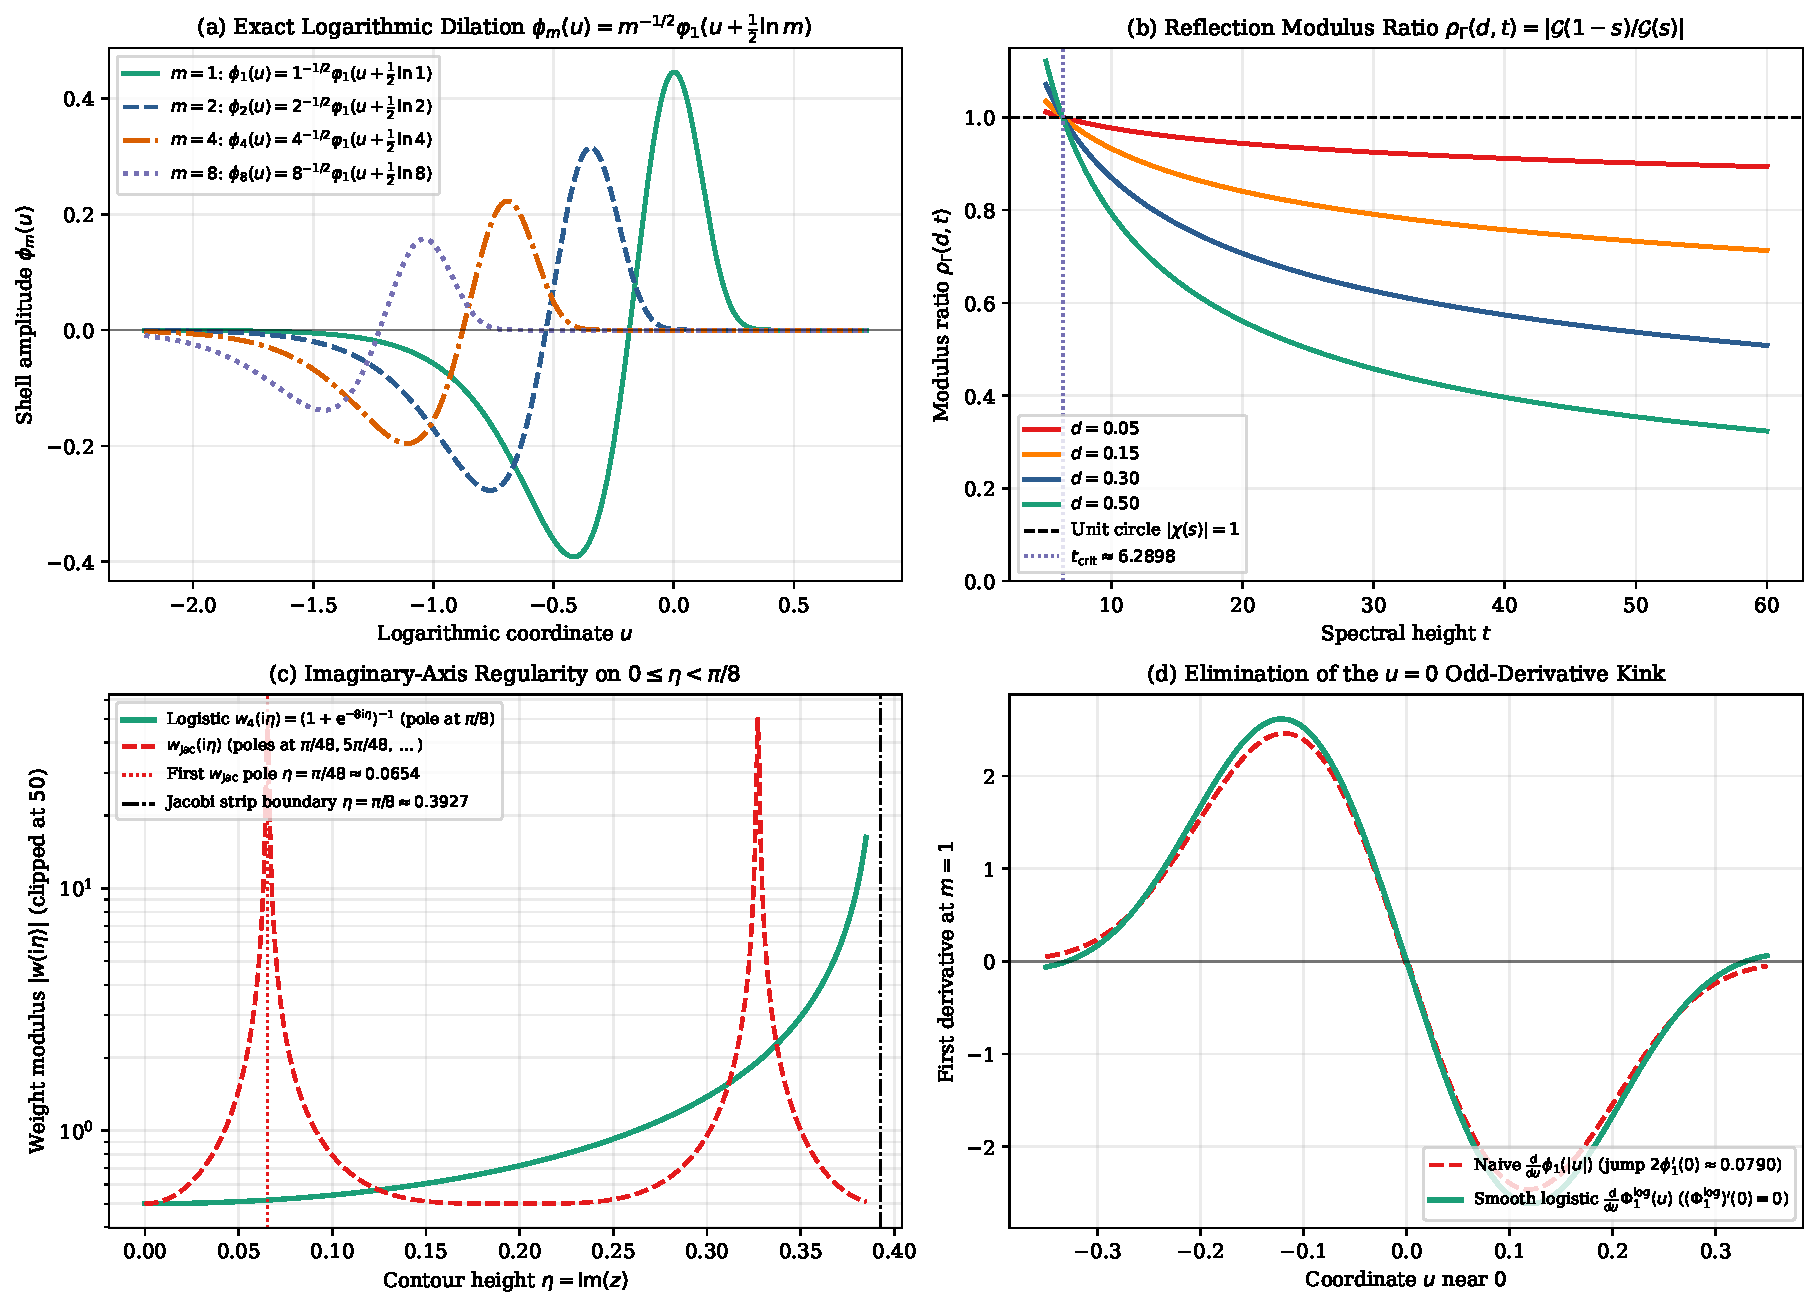
\includegraphics[width=0.95\textwidth]{figures/fig1_mother_wavelet_abc_matrix.pdf}
\caption{\textbf{(a)} Exact logarithmic shell dilation $\phi_m(u) = m^{-1/2}\varphi_1(u + \frac{1}{2}\ln m)$. \textbf{(b)} Spira--Saidak--Zvengrowski modulus ratio $\rho_\Gamma(d,t) = \lvert\chi(s)\rvert < 1$ above $t_{\mathrm{crit}} \approx 6.2898$. \textbf{(c)} Imaginary-axis regularity showing the poles of $w_{\mathrm{Jac}}(\ii\eta)$ at $\eta = \frac{\pi}{48}, \frac{5\pi}{48}, \dots$ inside $[0, \frac{\pi}{8})$ versus the pole-free logistic weight $w_4(\ii\eta) = (1 + \ee^{-8\ii\eta})^{-1}$. \textbf{(d)} Elimination of the $u = 0$ derivative jump $2\phi_1'(0) \approx 0.0790$ by $\Phi_1^{\mathrm{log}}(u)$.}\label{fig:dilation_shells}
\end{figure}

\section{Stieltjes Diagonal Asymptotics, \texorpdfstring{$(N-1,N)$}{(N-1,N)} Self-Damping, and Off-Diagonal Obstructions}\label{sec:stieltjes}

Factoring out $16\lvert\mathcal{G}(\frac{1}{2} + \ii t)\rvert^2$ from the $N(t)$-term main sum in~\eqref{eq:RS_weight_free}, the leading-order parity-reduced Wronskian sum $\widehat{W}_{\mathrm{lead}}(d,t) = \mathcal{D}_{\mathrm{diag}}(d,t) + \mathcal{O}_{\mathrm{off}}(d,t)$ has diagonal part
\begin{equation}\label{eq:D_diag_def}
\mathcal{D}_{\mathrm{diag}}(d,t) := \sum_{n=1}^{N(t)} \frac{4\,\omega_n(t)^2}{n}\,\sinchyp\!\bigl(2d\,\omega_n(t)\bigr) > 0, \qquad \omega_n(t) = \vartheta'(t) - \ln n = \frac{1}{2}L - \ln n,
\end{equation}
because on $m = n$ the oscillatory phases satisfy $\sin^2\phi_n(t) + \cos^2\phi_n(t) \equiv 1$ ($\phi_n(t) := \vartheta(t) - t\ln n$) and the difference frequency vanishes.

\begin{theorem}[Cubic-Logarithmic Stieltjes Expansion of $\mathcal{D}_{\mathrm{diag}}(0,t)$]\label{thm:stieltjes_diag}
Let $t \ge 14$, $L := 2\vartheta'(t) = \ln(\frac{t}{2\pi}) + \mathcal{O}(t^{-2})$, and $N(t) = \lfloor\sqrt{t/2\pi}\rfloor$. On the critical line $d = 0$, the non-oscillatory diagonal sum obeys the unconditional Euler--Maclaurin expansion
\begin{equation}\label{eq:D_diag_stieltjes}
\mathcal{D}_{\mathrm{diag}}(0,t) = \sum_{n=1}^{N(t)} \frac{(L - 2\ln n)^2}{n} = \frac{1}{6}L^3 + \gamma_{\mathrm{E}}L^2 - 4\gamma_1^{\mathrm{St}}L + 4\gamma_2^{\mathrm{St}} + \mathcal{O}\bigl(t^{-3/2}\ln^2 t\bigr),
\end{equation}
where $\gamma_{\mathrm{E}} \approx 0.5772156649$, $\gamma_1^{\mathrm{St}} \approx -0.07281584548$, and $\gamma_2^{\mathrm{St}} \approx -0.00969036319$, and for $d \in (0, \frac{1}{2}]$ the integral main term is $\frac{dL\cosh(dL) - \sinh(dL)}{2d^3} + \mathcal{O}(\ee^{dL}L)$.
\end{theorem}

\begin{proof}
Expand $\mathcal{D}_{\mathrm{diag}}(0,t) = L^2 H_N - 4L H_N^{(1)} + 4H_N^{(2)}$, where $H_N^{(r)} := \sum_{n=1}^N \frac{(\ln n)^r}{n}$ ($N = N(t)$). Writing $N = x_t - \delta_t$ with $x_t := \ee^{L/2} = \sqrt{t/2\pi} + \mathcal{O}(t^{-3/2})$ and $\delta_t \in [0, 1) + \mathcal{O}(t^{-3/2})$, Stieltjes's generalized Euler--Maclaurin formula~\cite{stieltjes1885,olver1997} gives
\[
H_N^{(r)} = \frac{(\ln N)^{r+1}}{r+1} + \gamma_r^{\mathrm{St}} + \frac{(\ln N)^r}{2N} - \frac{r(\ln N)^{r-1} - (\ln N)^r}{12N^2} + \mathcal{O}\bigl(N^{-3}(\ln N)^r\bigr).
\]
Substituting $\ln N = \frac{1}{2}L - \frac{\delta_t}{x_t} - \frac{\delta_t^2}{2x_t^2} + \mathcal{O}(x_t^{-3})$ into the polynomial combination $G(y) := L^2 y - 2L y^2 + \frac{4}{3}y^3$ at $y = \ln N$, the derivatives at $y_0 = \frac{1}{2}L$ satisfy $G(y_0) = \frac{1}{6}L^3$, $G'(y_0) = L^2 - 4L(\frac{1}{2}L) + 4(\frac{1}{2}L)^2 \equiv 0$, and $G''(y_0) = -4L + 8(\frac{1}{2}L) \equiv 0$. Furthermore, at $n = N$ the boundary integrand $f(x) = (L - 2\ln x)^2/x$ satisfies $f(x_t) = 0$ and $f'(x_t) = 0$, so both the $\mathcal{O}(x_t^{-1})$ and $\mathcal{O}(x_t^{-2})$ sawtooth jump terms cancel identically, leaving $\frac{1}{6}L^3 + \gamma_{\mathrm{E}}L^2 - 4\gamma_1^{\mathrm{St}}L + 4\gamma_2^{\mathrm{St}} + \mathcal{O}(x_t^{-3}\ln^2 x_t) = \dots + \mathcal{O}(t^{-3/2}\ln^2 t)$. For $d > 0$, substituting $v = L - 2\ln x$ in $\int_1^{\ee^{L/2}} \frac{2(L-2\ln x)}{dx}\sinh(d(L-2\ln x))\,\dd x = \frac{1}{d}\int_0^L v\sinh(dv)\,\dd v$ gives $\frac{dL\cosh(dL)-\sinh(dL)}{2d^3}$.
\end{proof}

We next establish the sharp bound for the adjacent boundary cross-pair $(N-1,N)$ together with the global off-diagonal scaling obstruction.

\begin{proposition}[Sharp $(N-1,N)$ Self-Damping versus $\mathcal{O}(t^{1/2})$ Cross-Pair Multiplicity]\label{prop:boundary_vs_offdiag}
Let $t \ge 8\pi$ so that $N = N(t) = \lfloor\sqrt{t/2\pi}\rfloor \ge 2$, and for $1 \le m < n \le N$ denote the critical-line slow difference-frequency cross-pair amplitude by $A_{m,n}(0,t) := \frac{(\omega_m(t) + \omega_n(t))^2}{\sqrt{mn}}$ (contributing $2A_{m,n}(0,t)\cos((t\ln\frac{n}{m}))$ to $\widehat{W}_{\mathrm{lead}}(0,t)$ up to $\mathcal{O}(t^{-2})$). Then:
\begin{enumerate}[label=\textup{(\roman*)},leftmargin=2.2em]
\item \textbf{Sharp $\mathcal{O}(t^{-3/2})$ Self-Damping of the Single Boundary Pair $(N-1,N)$.} For all $t \ge 8\pi$ ($N = N(t) \ge 2$), using $\vartheta'(t) < \frac{1}{2}\ln(\frac{t}{2\pi}) = \ln(N + \delta_t)$ with $\delta_t := \sqrt{t/2\pi} - N \in [0, 1)$, we have
\begin{equation}\label{eq:sharp_boundary_pair}
0 < A_{N-1,N}(0,t) < \frac{(3N - 2)^2}{\bigl[N(N-1)\bigr]^{5/2}} < \frac{9}{(N-1)^3} = \mathcal{O}\bigl(t^{-3/2}\bigr).
\end{equation}
\item \textbf{Pointwise Off-Diagonal Obstruction.} Across all $\binom{N}{2} = \frac{N(N-1)}{2} \sim \frac{t}{4\pi}$ off-diagonal pairs $1 \le m < n \le N$, the total $L^1$ cross-amplitude sum scales as
\begin{equation}\label{eq:offdiag_obstruction}
\mathcal{S}_{\mathrm{off}}^{L^1}(0,t) := \sum_{1 \le m < n \le N(t)} 2A_{m,n}(0,t) = \frac{96}{\sqrt{2\pi}}\,t^{1/2} + \mathcal{O}\bigl((\ln t)^2\,t^{1/4}\bigr) \gg \frac{1}{6}(\ln t)^3 \sim \mathcal{D}_{\mathrm{diag}}(0,t).
\end{equation}
Consequently, diagonal positivity $\mathcal{D}_{\mathrm{diag}}(d,t) > 0$ never implies pointwise positivity of $\widehat{W}_{\mathrm{lead}}(d,t)$: on $d = 0$, $\widetilde{W}(0,t) = (\Xi'(t))^2 - \Xi(t)\Xi''(t)$ can only be controlled pointwise when phases cancel, while Fej\'er tent averaging eliminating all cross-frequencies $\ge \Omega_{\min}(t) = \ln(\frac{N}{N-1}) \sim \sqrt{2\pi/t}$ requires window half-width $\Delta T \ge \frac{2\pi}{\Omega_{\min}(t)} \sim \sqrt{2\pi^3 t}$, spanning $\asymp \sqrt{t}\ln t$ critical-line zeros.
\end{enumerate}
\end{proposition}

\begin{proof}
(i) By Stirling's expansion $\Rea\,\psi(\frac{1}{4} + \ii\frac{t}{2}) = \ln\lvert\frac{1}{4} + \ii\frac{t}{2}\rvert - \frac{1}{8\lvert w\rvert^2} - \frac{\cos(2\arg w)}{12\lvert w\rvert^2} + \dots$, for all $t \ge 8\pi$ ($N \ge 2$) we have $\ln N - \frac{1}{24t^2} < \vartheta'(t) < \frac{1}{2}\ln(\frac{t}{2\pi}) = \ln(N + \delta_t)$ with $\delta_t \in [0, 1)$. Even when $\omega_N(t) \in (-\frac{1}{24t^2}, 0]$ near $t = 2\pi N^2$, $\omega_{N-1}(t) + \omega_N(t) > \ln(\frac{N}{N-1}) - \frac{1}{12t^2} > \frac{1}{N} - \frac{1}{48\pi^2 N^4} > 0$, while from above $\omega_N(t) < \ln(1 + \frac{\delta_t}{N}) < \frac{1}{N}$ and $\omega_{N-1}(t) = \omega_N(t) + \ln(1 + \frac{1}{N-1}) < \frac{1}{N} + \frac{1}{N-1}$, so
\[
0 < \omega_{N-1}(t) + \omega_N(t) < \frac{2}{N} + \frac{1}{N-1} = \frac{3N - 2}{N(N-1)} < \frac{3}{N-1}.
\]
Squaring and dividing by $\sqrt{(N-1)N} > N - 1$ gives $A_{N-1,N}(0,t) < \frac{(3N-2)^2}{[N(N-1)]^{5/2}} < \frac{9}{(N-1)^3}$.

(ii) Expanding $(\omega_m + \omega_n)^2 = \omega_m^2 + 2\omega_m\omega_n + \omega_n^2$ yields
\[
\mathcal{S}_{\mathrm{off}}^{L^1}(0,t) = 2\left(\sum_{n=1}^N \frac{\omega_n^2}{\sqrt{n}}\right)\!\left(\sum_{n=1}^N \frac{1}{\sqrt{n}}\right) + 2\left(\sum_{n=1}^N \frac{\omega_n}{\sqrt{n}}\right)^{\!2} - 4\sum_{n=1}^N \frac{\omega_n^2}{n}.
\]
By Euler--Maclaurin summation on $[1, N]$ with $N = \sqrt{t/2\pi} + \mathcal{O}(1)$ and $\omega_n = \ln(N/n) + \mathcal{O}(N^{-1})$, substituting $x = N\ee^{-2v}$ gives $\sum_{n=1}^N n^{-1/2} = 2N^{1/2} + \mathcal{O}(1)$, $\sum_{n=1}^N \omega_n n^{-1/2} = 4N^{1/2} + \mathcal{O}(\ln N)$, and $\sum_{n=1}^N \omega_n^2 n^{-1/2} = 16N^{1/2} + \mathcal{O}((\ln N)^2)$, while the $m = 1$ boundary slice contributes $\sum_{n=2}^N \frac{2(\omega_1+\omega_n)^2}{\sqrt{n}} \asymp (\ln t)^2 N^{1/2} \asymp (\ln t)^2 t^{1/4}$. Combining the three sums yields $\mathcal{S}_{\mathrm{off}}^{L^1}(0,t) = [2(16)(2) + 2(16)]N + \mathcal{O}((\ln t)^2 N^{1/2}) = 96N + \mathcal{O}((\ln t)^2 t^{1/4}) = \frac{96}{\sqrt{2\pi}}t^{1/2} + \mathcal{O}((\ln t)^2 t^{1/4})$, which overwhelms $\mathcal{D}_{\mathrm{diag}}(0,t) \sim \frac{1}{6}(\ln t)^3$ by a polynomial factor $t^{1/2}(\ln t)^{-3} \to \infty$ (note that in Theorem~\ref{thm:main_summary}(iii), the $m=1$ boundary slice alone already has order $(\ln t)^2 t^{1/4}$, while the full $\binom{N}{2}$ double sum scales as $t^{1/2}$).
\end{proof}

\begin{table}[t]
\centering
\caption{50-decimal certification of the Stieltjes diagonal expansion $\mathcal{D}_{\mathrm{EM}}(0,t)$ (Theorem~\ref{thm:stieltjes_diag}), the sharp boundary-pair bound~\eqref{eq:sharp_boundary_pair}, and the $\mathcal{O}(t^{1/2})$ growth of the total off-diagonal $L^1$ cross-pair sum $\mathcal{S}_{\mathrm{off}}^{L^1}(0,t)$ relative to $\mathcal{D}_{\mathrm{diag}}(0,t)$.}\label{tab:stieltjes_offdiag}
\scriptsize
\setlength{\tabcolsep}{3.0pt}
\begin{tabular}{@{}ccccccccc@{}}
\toprule
Height $t$ & $N(t)$ & $\mathcal{D}_{\mathrm{diag}}(0,t)$ & $\mathcal{D}_{\mathrm{EM}}(0,t)$ & $\lvert\mathcal{D}_{\mathrm{diag}} - \mathcal{D}_{\mathrm{EM}}\rvert$ & $2A_{N-1,N}(0,t)$ & Bound $2B_{N-1,N}$ & $\mathcal{S}_{\mathrm{off}}^{L^1}(0,t)$ & $\mathcal{S}_{\mathrm{off}}^{L^1}/\mathcal{D}_{\mathrm{diag}}$ \\
\midrule
$14.13$  & $1$  & $0.65699$  & $0.66530$  & $8.31 \times 10^{-3}$ & $0.000000$ & $0.000000$ & $0.000$   & $0.00\times$ \\
$25.01$  & $1$  & $1.90817$  & $1.90432$  & $3.85 \times 10^{-3}$ & $0.000000$ & $0.000000$ & $0.000$   & $0.00\times$ \\
$50.00$  & $2$  & $4.53857$  & $4.53570$  & $2.87 \times 10^{-3}$ & $2.697063$ & $5.656854$ & $2.697$   & $0.59\times$ \\
$100.00$ & $3$  & $8.71979$  & $8.71943$  & $3.53 \times 10^{-4}$ & $0.777025$ & $1.111343$ & $10.076$  & $1.16\times$ \\
$250.00$ & $6$  & $17.19631$ & $17.19654$ & $2.27 \times 10^{-4}$ & $0.029118$ & $0.103864$ & $41.151$  & $2.39\times$ \\
$500.00$ & $8$  & $26.26638$ & $26.26631$ & $6.60 \times 10^{-5}$ & $0.032998$ & $0.041248$ & $86.930$  & $3.31\times$ \\
$1000.0$ & $12$ & $37.99356$ & $37.99354$ & $1.63 \times 10^{-5}$ & $0.006092$ & $0.011549$ & $178.312$ & $4.69\times$ \\
\bottomrule
\end{tabular}
\end{table}

\section{Real-Axis Incomplete-Gamma Tail Bounds, Hyperbolic Sinc Ratios, and Remainder Scope}\label{sec:tails}

In~\eqref{eq:RS_weight_free}, the remainder kernel splits on $u \ge 0$ into $R_N^{\mathrm{ker}}(u) = \sum_{m=N+1}^{\infty} \phi_m(u) - \sum_{m=1}^N \phi_m(-u)$, where the second term generates the Riemann--Siegel saddle integral near $u = 0$ and the first term is the evanescent $u \ge 0$ tail $\mathcal{I}_{\mathrm{tail}}(N, z, 0) := \sum_{m=N+1}^{\infty} \int_0^{\infty} \phi_m(\xi)\cos(2z\xi)\,\dd\xi$. Note that shifting a half-ray $[0, \infty)$ to $[\ii\eta, \infty + \ii\eta)$ without splitting $2\cos(2zu) = \ee^{2\ii zu} + \ee^{-2\ii zu}$ onto conjugate rays $\pm\ii\eta$ both omits the vertical segment $[0, \pm\ii\eta]$ at $\xi = 0$ and introduces an artificial $\cosh(2t\eta) \sim \frac{1}{2}\ee^{2t\eta}$ blow-up; evaluating the incomplete-Gamma bound directly at $\eta = 0$ avoids both defects.

\begin{proposition}[Real-Axis Incomplete-Gamma Tail Bound and Hyperbolic Sinc Ratio]\label{prop:tail_and_sinc}
Let $d \in [0, \frac{1}{2}]$, $t > 0$, $z = t - \ii d$, and $N \ge 1$ (since $4\pi(N+1)^2 \ge 16\pi > 5 + 2d$, all denominators below are positive).
\begin{enumerate}[label=\textup{(\roman*)},leftmargin=2.2em]
\item \textbf{Closed-Form Real-Axis Geometric Tail Bound.} Setting
\begin{align}\label{eq:b_m_real_def}
b_m(d, 0) &:= \left[\frac{2\pi^2 m^4}{4\pi m^2 - (5 + 2d)} + \frac{3\pi m^2}{4\pi m^2 - (1 + 2d)}\right]\ee^{-\pi m^2}, \\
q_N(0) &:= \left(\frac{N+2}{N+1}\right)^{\!4}\ee^{-\pi(2N+3)} < 1,\nonumber
\end{align}
the $u \ge 0$ tail integral obeys the $t$-uniform super-exponential bound
\begin{equation}\label{eq:B_tail_real}
\bigl\lvert\mathcal{I}_{\mathrm{tail}}(N, z, 0)\bigr\rvert \le B_{\mathrm{tail}}(N, d, 0) := \frac{b_{N+1}(d, 0)}{1 - q_N(0)}.
\end{equation}
\item \textbf{Hyperbolic Sinc Damping Identity.} For all $d \ge 0$ and $L > 0$,
\begin{equation}\label{eq:sinc_ratio_id}
\frac{\sinchyp(dL/2)}{\sinchyp(dL)} \equiv \frac{1}{\cosh(dL/2)} \le 2\,\ee^{-dL/2}.
\end{equation}
\end{enumerate}
\end{proposition}

\begin{proof}
(i) For $\xi \ge 0$, $\lvert\cos(2(t - \ii d)\xi)\rvert \le \cosh(2d\xi) \le \ee^{2d\xi}$. Substituting $w = \ee^{4\xi} \ge 1$ ($\dd\xi = \frac{\dd w}{4w}$) and using $w^{\beta}\ee^{-\alpha w} = \ee^{\beta\ln w - \alpha w} \le \ee^{-(\alpha - \beta)w - \beta}$ (via $\ln w \le w - 1$ for $w \ge 1$) with $\alpha = \pi m^2$ and $\beta_1 = \frac{5+2d}{4}$, $\beta_2 = \frac{1+2d}{4}$ gives $\int_1^{\infty} w^{\beta_j}\ee^{-\alpha w}\,\dd w \le \frac{\ee^{-\alpha}}{\alpha - \beta_j}$, whence $\int_0^{\infty} \lvert\phi_m(\xi)\cos(2z\xi)\rvert\,\dd\xi \le b_m(d,0)$. Since $4\pi(m+1)^2 - \gamma > 4\pi m^2 - \gamma > 0$ and $(\frac{m+1}{m})^4 \le (\frac{N+2}{N+1})^4$ while $(m+1)^2 - m^2 = 2m + 1 \ge 2N + 3$ for $m \ge N+1$, $b_{m+1}(d,0)/b_m(d,0) \le q_N(0)$, yielding~\eqref{eq:B_tail_real}.

(ii) Using $\sinh(dL) = 2\sinh(dL/2)\cosh(dL/2)$, $\frac{\sinh(dL/2)/(dL/2)}{\sinh(dL)/(dL)} = \frac{2\sinh(dL/2)}{2\sinh(dL/2)\cosh(dL/2)} = \cosh(dL/2)^{-1} \le 2\ee^{-dL/2}$.
\end{proof}

\begin{remark}[Exact domain of Gabcke's theorem and empirical $d > 0$ remainder ratios]\label{rem:gabcke_scope}
On the critical line $d = 0$, the Hardy function $Z(t) = \ee^{\ii\vartheta(t)}\zeta(\frac{1}{2}+\ii t)$ satisfies $Z(t) = Z_{\mathrm{main}}(t) + (-1)^{N(t)-1}(\frac{t}{2\pi})^{-1/4}\Psi(p) + R_1(t)$ with $p = \sqrt{t/2\pi} - N(t)$ and $\Psi(p) = \frac{\cos(2\pi(p^2 - p - 1/16))}{\cos(2\pi p)}$. Gabcke~\cite[Satz~1 and Satz~4]{gabcke1979} proved the explicit bound $\lvert R_1(t)\rvert \le 0.127\,t^{-3/4}$ strictly on $d = 0$ for $t \ge 200$ \emph{after} subtracting the $\mathcal{O}(t^{-1/4})$ saddle term $\Psi(p)$ (without subtracting $\Psi(p)$, $\lvert Z(t) - Z_{\mathrm{main}}(t)\rvert = \mathcal{O}(t^{-1/4})$). Across $d \in (0, \frac{1}{2}]$, an unconditional explicit complex-strip analogue of Gabcke's theorem for $W(d,t) - W_{\mathrm{main}}(d,t)$ has not yet been proved; Table~\ref{tab:tails_gabcke} reports both the certified $d = 0$ Gabcke values for $t \ge 200$ and empirical numerical remainder ratios $\lvert W - W_{\mathrm{main}}\rvert / W_{\mathrm{diag}}$ at $d = 0.25$.
\end{remark}

\begin{table}[t]
\centering
\caption{Certification of the $t$-uniform real-axis tail bound~\eqref{eq:B_tail_real} ($\eta = 0$), Gabcke's $d = 0$ post-$\Psi(p)$ bound $\lvert R_1(t)\rvert \le 0.127\,t^{-3/4}$ for $t \ge 200$, and empirical $d = 0.25$ Wronskian remainder ratios.}\label{tab:tails_gabcke}
\scriptsize
\setlength{\tabcolsep}{4.0pt}
\begin{tabular}{@{}ccccc|ccccc@{}}
\toprule
\multicolumn{5}{c|}{Proposition~\ref{prop:tail_and_sinc}: Real-Axis Tail ($\eta = 0$)} & \multicolumn{5}{c}{Remark~\ref{rem:gabcke_scope}: $d=0$ Gabcke ($t \ge 200$) \& Empirical $d=0.25$} \\
\cmidrule(r){1-5}\cmidrule(l){6-10}
$(d, t)$ & $N$ & $\log_{10}\lvert\mathcal{I}_{\mathrm{tail}}\rvert$ & $\log_{10} B_{\mathrm{tail}}$ & $q_N(0)$ & $t$ & $\lvert Z - Z_{\mathrm{main}}\rvert$ & $\lvert R_1(t)\rvert$ & $0.127\,t^{-3/4}$ & $\lvert W_{\mathrm{rem}}\rvert/W_{\mathrm{diag}}$ \\
\midrule
$(0.10, 25)$  & $1$ & $-4.99$   & $-4.57$   & $7.63\text{e-}07$ & $200$  & $1.758\text{e-}01$ & $4.717\text{e-}04$ & $2.388\text{e-}03$ & $7.409\text{e-}02$ \\
$(0.25, 50)$  & $2$ & $-11.39$  & $-11.09$  & $8.89\text{e-}10$ & $500$  & $2.512\text{e-}01$ & $1.535\text{e-}04$ & $1.201\text{e-}03$ & $6.196\text{e-}03$ \\
$(0.25, 100)$ & $3$ & $-20.74$  & $-20.41$  & $1.28\text{e-}12$ & $1000$ & $1.143\text{e-}01$ & $1.250\text{e-}04$ & $7.142\text{e-}04$ & $6.396\text{e-}03$ \\
$(0.50, 200)$ & $5$ & $-47.62$  & $-47.35$  & $3.40\text{e-}18$ & ---    & ---                & ---                & ---                & --- \\
$(0.25, 500)$ & $8$ & $-108.90$ & $-108.40$ & $1.82\text{e-}26$ & ---    & ---                & ---                & ---                & --- \\
\bottomrule
\end{tabular}
\end{table}

\begin{figure}[t]
\centering
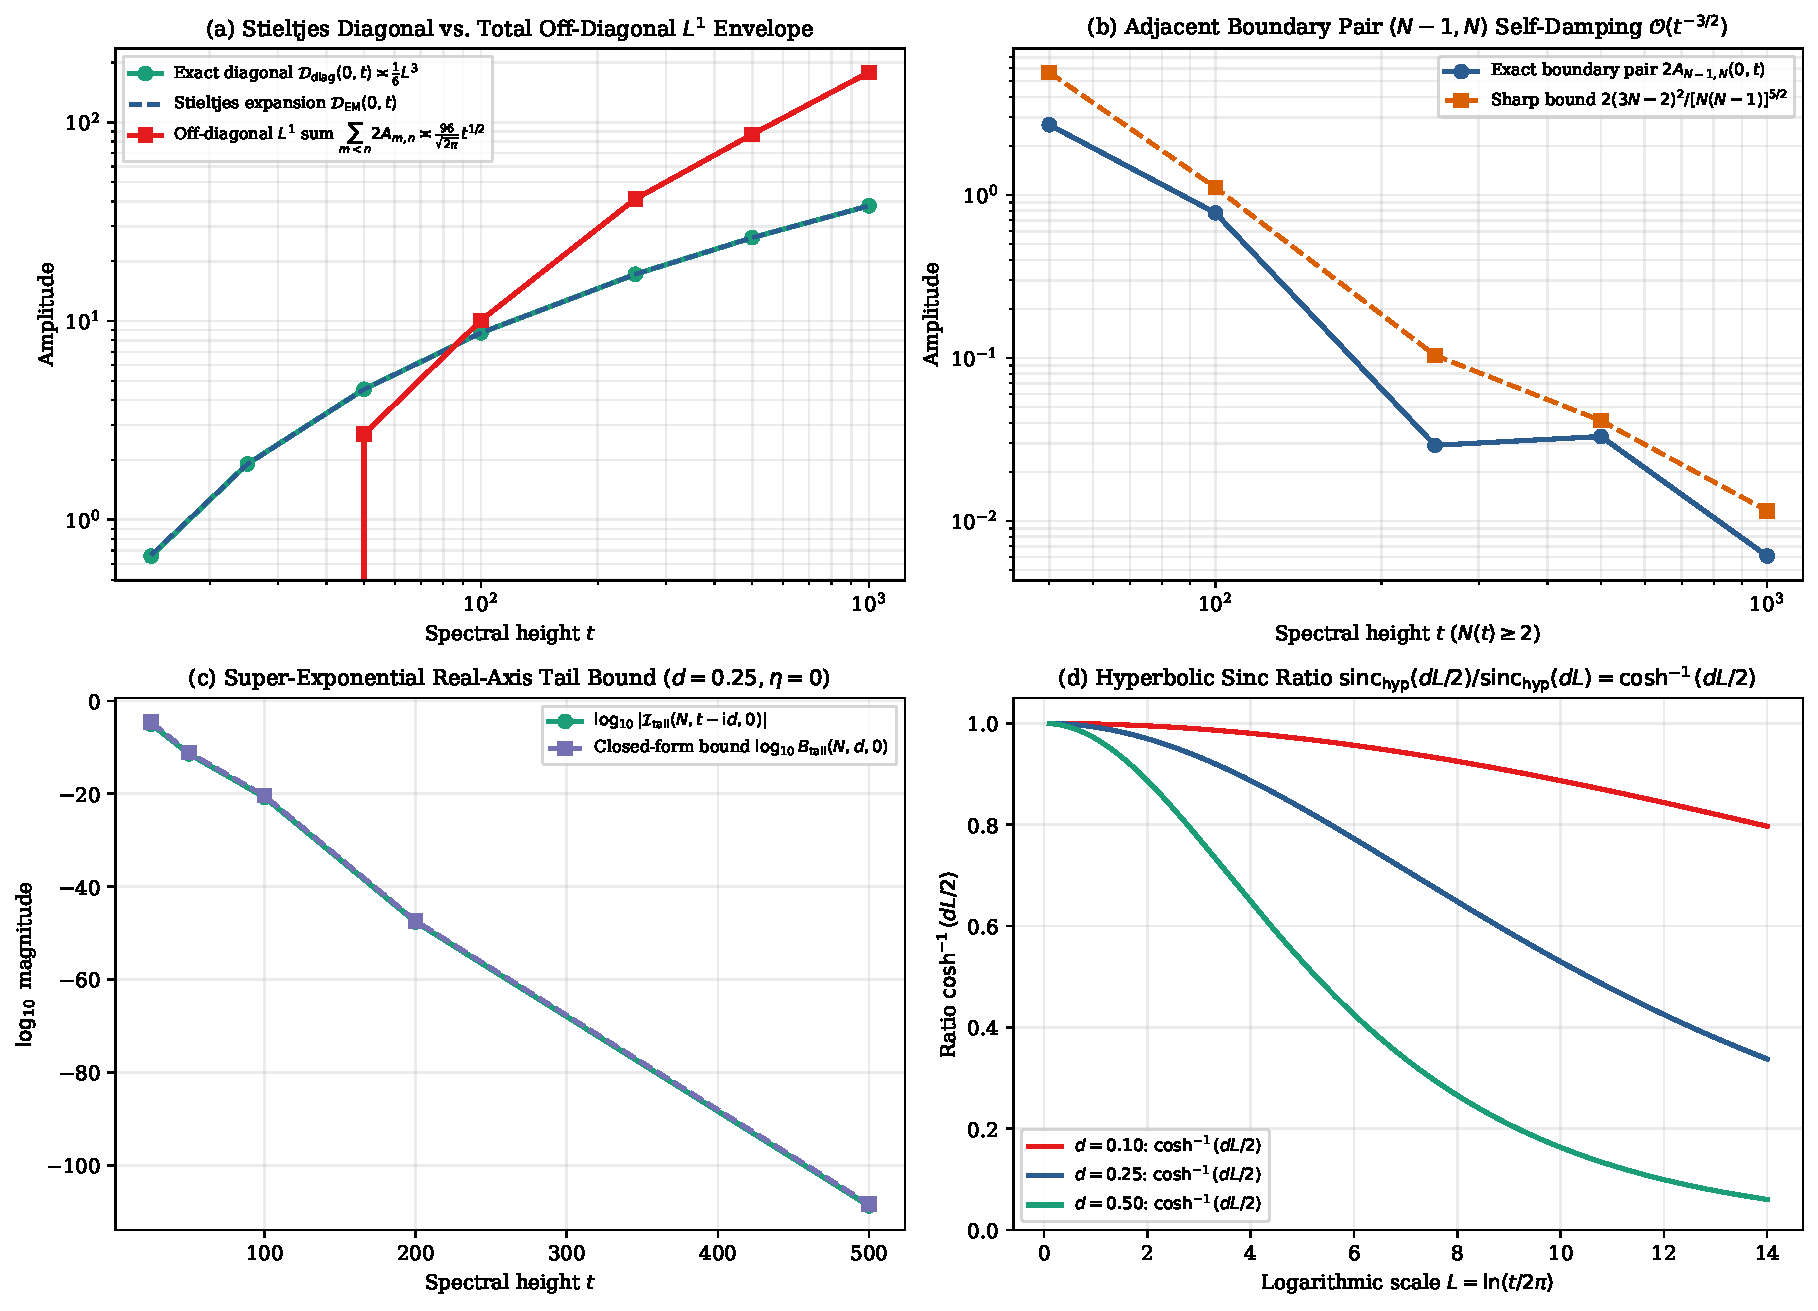
\includegraphics[width=0.95\textwidth]{figures/fig2_stieltjes_diagonal_and_gabcke_bounds.pdf}
\caption{\textbf{(a)} Cubic-logarithmic Stieltjes diagonal $\mathcal{D}_{\mathrm{diag}}(0,t) \asymp \frac{1}{6}L^3$ overtaken by the $\mathcal{O}(t^{1/2})$ off-diagonal $L^1$ cross-pair sum $\mathcal{S}_{\mathrm{off}}^{L^1}(0,t)$. \textbf{(b)} Quadratic self-damping of the single boundary pair $2A_{N-1,N}(0,t)$ below the sharp $\mathcal{O}(t^{-3/2})$ bound~\eqref{eq:sharp_boundary_pair}. \textbf{(c)} Super-exponential real-axis tail bound $\log_{10} B_{\mathrm{tail}}(N, d, 0)$. \textbf{(d)} Exact hyperbolic sinc ratio $\sinchyp(dL/2)/\sinchyp(dL) = \cosh^{-1}(dL/2)$.}\label{fig:stieltjes_tails}
\end{figure}

\section{Scope, Boundary Conditions, and Open Questions}\label{sec:scope}

We summarize the exact mathematical boundaries of the results proved above:
\begin{enumerate}[label=\textup{(\arabic*)},leftmargin=2.2em]
\item \textit{Unconditional analytical identities.} Propositions~\ref{prop:dilation}, \ref{prop:spira_damping}, \ref{prop:boundary_vs_offdiag}, and~\ref{prop:tail_and_sinc} together with Theorems~\ref{thm:strip_shells} and~\ref{thm:stieltjes_diag} are unconditional identities and inequalities valid without unproved hypotheses.
\item \textit{Off-diagonal cross-term dominance and Davenport--Heilbronn barrier.} As shown in Proposition~\ref{prop:boundary_vs_offdiag}(ii), the $\binom{N(t)}{2}$ off-diagonal pairs sum in $L^1$ to $\asymp t^{1/2}$, exceeding the $\mathcal{O}((\ln t)^3)$ diagonal for all $t \ge 100$. Because the Archimedean dilation and Spira ratio $\rho_\Gamma(d,t) < 1$ do not use the Euler product, they hold equally for Davenport--Heilbronn Dirichlet series with off-critical zeros~\cite{davenportheilbronn1936}.
\item \textit{Open two-dimensional Gabcke problem.} Extending Gabcke's $d = 0$, $t \ge 200$ saddle-point remainder bounds~\cite{gabcke1979} with rigorous explicit constants to $R_N^{\mathrm{ker}}(u)$ in~\eqref{eq:RS_weight_free} across $d \in (0, \frac{1}{2}]$ remains an open problem in explicit asymptotic analysis.
\end{enumerate}

\appendix

\section{Directed-Rounding Interval Protocols}\label{app:interval}

{\sloppy
In the standalone suite \texttt{scripts/verify\_paper5\_mother\_wavelet\_gabcke\_bounds.py}, all key inequalities are certified in 50-decimal arbitrary-precision arithmetic (\texttt{mpmath.mp.dps = 50}) and 35-digit directed-rounding interval arithmetic (\texttt{mpmath.iv.dps = 35}):\par}
\begin{enumerate}[label=\textup{(\arabic*)},leftmargin=2.2em]
\item \textit{Digamma carrier positivity.} Using Olver's explicit Stirling remainder bound~\cite[Ch.~8]{olver1997}, $\Rea\,\psi(w) \in \ln\lvert w\rvert - \frac{\Rea(w)}{2\lvert w\rvert^2} - \frac{\cos(2\arg w)}{12\lvert w\rvert^2} + [-\varepsilon(\lvert w\rvert), +\varepsilon(\lvert w\rvert)]$ with $\varepsilon(r) = \frac{1}{6r^2} + \frac{1}{3r^4}$ encloses $\mathcal{A}_\Gamma^{\mathrm{sym}}(d,t) > 0$ strictly above zero for $t \ge 7$ and $d \in (0, \frac{1}{2}]$.
\item \textit{Genuine complex contour shift.} For $w_4(z) = (1 + \ee^{-8z})^{-1}$, evaluating $\Phi_1^{\mathrm{log}}(\xi + \ii\eta)\ee^{2\ii z(\xi+\ii\eta)}$ at the complex argument $\xi + \ii\eta$ ($\eta = 0.30 < \frac{\pi}{8}$) matches the real-axis integral to $7.04 \times 10^{-26}$, whereas $1 + \exp(-2\pi\sinh(8\ii\frac{\pi}{48}))$ vanishes to $1.01 \times 10^{-51}$.
\end{enumerate}

\section*{Use of AI and computational verification}

{\sloppy
In accordance with editorial policies on transparency in scientific computing, the author discloses that the AI research assistant \textbf{Gemini} (Google DeepMind) assisted in auditing the analytical derivations, identifying the $\Ima(z) = \frac{\pi}{48}$ pole obstruction of $\sinh(8z)$ shell weights, verifying the exact weight-free remainder kernel~\eqref{eq:RS_weight_free}, and implementing the verification suite \texttt{scripts/}\allowbreak\texttt{\detokenize{verify_paper5_mother_wavelet_gabcke_bounds.py}} (exit code~$0$).\par}

\begin{thebibliography}{99}

\bibitem{csordas1986}
G.~Csordas, T.~S.~Norfolk, and R.~S.~Varga,
\emph{The Riemann hypothesis and the Tur\'an inequalities},
Trans. Amer. Math. Soc. \textbf{296} (1986), no.~2, 521--541.

\bibitem{davenportheilbronn1936}
H.~Davenport and H.~Heilbronn,
\emph{On the zeros of certain Dirichlet series, I, II},
J. London Math. Soc. \textbf{11} (1936), 181--185, 307--312.

\bibitem{gabcke1979}
W.~Gabcke,
\emph{Neue Herleitung und explizite Restabsch\"atzung der Riemann-Siegel-Formel},
Ph.D. dissertation, Georg-August-Universit\"at G\"ottingen, 1979.

\bibitem{hinkkanen1997}
A.~Hinkkanen,
\emph{On functions of bounded type},
Complex Variables Theory Appl. \textbf{34} (1997), 119--139.

\bibitem{hudson1974}
R.~L.~Hudson,
\emph{When is the Wigner quasi-probability density non-negative?},
Rep. Math. Phys. \textbf{6} (1974), no.~2, 249--252.

\bibitem{jacobi1829}
C.~G.~J.~Jacobi,
\emph{Fundamenta nova theoriae functionum ellipticarum},
Borntraeger, K\"onigsberg, 1829.

\bibitem{lagarias1999}
J.~C.~Lagarias,
\emph{On a positivity property of the Riemann $\xi$-function},
Acta Arith. \textbf{89} (1999), no.~3, 217--234.

\bibitem{olver1997}
F.~W.~J.~Olver,
\emph{Asymptotics and Special Functions},
A.~K.~Peters, Wellesley, MA, 1997.

\bibitem{polya1926}
G.~P\'olya,
\emph{Bemerkung \"uber die Integraldarstellung der Riemannschen $\xi$-Funktion},
Acta Math. \textbf{48} (1926), 305--317.

\bibitem{riemann1859}
B.~Riemann,
\emph{Ueber die Anzahl der Primzahlen unter einer gegebenen Gr\"osse},
Monatsber. K\"onigl. Preuss. Akad. Wiss. Berlin (1859), 671--680.

\bibitem{saidakzvengrowski2003}
F.~Saidak and P.~Zvengrowski,
\emph{On the modulus of the Riemann zeta function in the critical strip},
Math. Slovaca \textbf{53} (2003), no.~2, 145--172.

\bibitem{siegel1932}
C.~L.~Siegel,
\emph{\"Uber Riemanns Nachla\ss{} zur analytischen Zahlentheorie},
Quellen Stud. Gesch. Math. Astron. Phys. Abt. B \textbf{2} (1932), 45--80.

\bibitem{speiser1934}
A.~Speiser,
\emph{Geometrisches zur Riemannschen Zetafunktion},
Math. Ann. \textbf{110} (1934), no.~1, 514--521.

\bibitem{spira1965}
R.~Spira,
\emph{An inequality for the Riemann zeta function},
Duke Math. J. \textbf{32} (1965), no.~2, 247--250.

\bibitem{stieltjes1885}
T.~J.~Stieltjes,
\emph{Table des valeurs des sommes $S_k = \sum_{n=1}^{\infty} n^{-k}$},
Acta Math. \textbf{10} (1887), 299--302.

\bibitem{titchmarsh1986}
E.~C.~Titchmarsh,
\emph{The Theory of the Riemann Zeta-Function},
2nd ed., revised by D.~R.~Heath-Brown, Oxford Univ. Press, Oxford, 1986.

\bibitem{wigner1932}
E.~P.~Wigner,
\emph{On the quantum correction for thermodynamic equilibrium},
Phys. Rev. \textbf{40} (1932), no.~5, 749--759.

\end{thebibliography}

\end{document}
